
% ----------------------------------------------------------------------
%  Set the document class
% ----------------------------------------------------------------------
\documentclass[11pt,a4paper,twoside]{article}

% ----------------------------------------------------------------------
% Define external packages, language, margins, fonts and new commands
% ----------------------------------------------------------------------
%\input{preamble} 
\usepackage[utf8]{inputenc}   % <<<<< Linux
\usepackage[english]{babel} % <<<<< English
\usepackage{notoccite}
\usepackage[skip=0.5\baselineskip]{caption}
\hyphenation{GTKWave}
\usepackage{listings}
\usepackage[all]{nowidow}

%blind text
\usepackage{lipsum}

\usepackage{graphicx}
\graphicspath{ {./} {../../figlib/} }
\def\FontLn{% 16 pt normal
  \usefont{T1}{phv}{m}{n}\fontsize{16pt}{16pt}\selectfont}
\def\FontLb{% 16 pt bold
  \usefont{T1}{phv}{b}{n}\fontsize{16pt}{16pt}\selectfont}
\def\FontMn{% 14 pt normal
  \usefont{T1}{phv}{m}{n}\fontsize{14pt}{14pt}\selectfont}
\def\FontMb{% 14 pt bold
  \usefont{T1}{phv}{b}{n}\fontsize{14pt}{14pt}\selectfont}
\def\FontSn{% 12 pt normal
  \usefont{T1}{phv}{m}{n}\fontsize{12pt}{12pt}\selectfont}

% Use Arial font as default
%
\renewcommand{\rmdefault}{phv}
\renewcommand{\sfdefault}{phv}
\usepackage{geometry}	
\geometry{verbose,tmargin=2.5cm,bmargin=2.5cm,lmargin=2.5cm,rmargin=2.5cm}

%\usepackage{setspace}
%\renewcommand{\baselinestretch}{1.5}

\usepackage[pdftex]{hyperref} % enhance documents that are to be
                              % output as HTML and PDF
\hypersetup{colorlinks,       % color text of links and anchors,
                              % eliminates borders around links
%            linkcolor=red,    % color for normal internal links
            linkcolor=black,  % color for normal internal links
            anchorcolor=black,% color for anchor text
%            citecolor=green,  % color for bibliographical citations
            citecolor=black,  % color for bibliographical citations
%            filecolor=magenta,% color for URLs which open local files
            filecolor=black,  % color for URLs which open local files
%            menucolor=red,    % color for Acrobat menu items
            menucolor=black,  % color for Acrobat menu items
%            pagecolor=red,    % color for links to other pages
            pagecolor=black,  % color for links to other pages
%            urlcolor=cyan,    % color for linked URLs
            urlcolor=black,   % color for linked URLs
	          bookmarks=true,         % create PDF bookmarks
	          bookmarksopen=false,    % don't expand bookmarks
	          bookmarksnumbered=true, % number bookmarks
	          pdftitle={report},
            pdfauthor={Andre C. Marta},
%            pdfsubject={Thesis Title},
%            pdfkeywords={Thesis Keywords},
            pdfstartview=FitV,
            pdfdisplaydoctitle=true}

\usepackage[numbers,sort&compress]{natbib} % <<<<< References in numbered list [1],[2],...
\usepackage{subcaption} 
\usepackage{mdframed}
\usepackage{amsmath}
\usepackage{placeins}
%%%%%%%%%%%%%%%%%%%%%%%%%%%%%%%%%%%%%%%%%%%%%%%%%%%%%%%%%%%%%%%%%%%%%%%%
%     Begin Document                                                   %
%%%%%%%%%%%%%%%%%%%%%%%%%%%%%%%%%%%%%%%%%%%%%%%%%%%%%%%%%%%%%%%%%%%%%%%%


\begin{document}

% Set plain page style (no headers, footer with centered page number)
\pagestyle{plain}

% Set roman numbering (i,ii,...) before the start of chapters
%\pagenumbering{roman}

% ----------------------------------------------------------------------
%  Cover page
% ----------------------------------------------------------------------
%%%%%%%%%%%%%%%%%%%%%%%%%%%%%%%%%%%%%%%%%%%%%%%%%%%%%%%%%%%%%%%%%%%%%%%%
%                                                                      %
%     File: Thesis_FrontCover.tex                                      %
%     Tex Master: Thesis.tex                                           %
%                                                                      %
%     Author: Andre C. Marta                                           %
%     Last modified :  2 Jul 2015                                      %
%                                                                      %
%%%%%%%%%%%%%%%%%%%%%%%%%%%%%%%%%%%%%%%%%%%%%%%%%%%%%%%%%%%%%%%%%%%%%%%%

\thispagestyle {empty}

% IST Logo - Signature A
% parameters: bb=llx lly urx ury (bounding box), width=h_length, height=v_length, angle=angle, scale=factor, clip=true/false, draft=true/false. 
\includegraphics[bb=9.5cm 11cm 0cm 0cm,scale=0.29]{IST_A_CMYK_POS}

\begin{center}
%
% Figure (Image or plot)
\vspace{1.0cm}
% height = 50 mm
%\includegraphics[height=50mm]{Figures/Airbus_A350.jpg}

% Title, author and degree
\vspace{1cm}
{\FontLb Circuit Theory and Electronics Fundamentals} \\ % <<<<< EDIT TITLE
\vspace{1cm}
{\FontSn Department of Electrical and Computer Engineering, Técnico, University of Lisbon} \\ % <<<<< EDIT COURSE
\vspace{1cm}
{\FontSn Laboratory Report} \\ 
\vspace{1cm} 
{\FontSn João Delile nº95800} 

\vspace{0.5cm}
{\FontSn José Murteira nº96547}

\vspace {0.5cm}
{\FontSn Manuel Candeias nº97259} 

\vspace{1cm}
{\FontSn March 22, 2021} \\ % <<<<< EDIT DATE (corresponds to date of oral examination)
%
\end{center}



% ----------------------------------------------------------------------
% Dedication page (optional)
% ----------------------------------------------------------------------
%\input{dedication} 
%\cleardoublepage

% ----------------------------------------------------------------------
%  Acknowledgments (optional)
% ----------------------------------------------------------------------
%\input{acknowledgements}
%\cleardoublepage

% ----------------------------------------------------------------------
%  Abstract (both in English and Portuguese)
% ----------------------------------------------------------------------
%\input{resumo} 
%\cleardoublepage

%\input{abstract} 

% ----------------------------------------------------------------------
%  Table of contents, list of tables, list of figures and nomenclature
% ----------------------------------------------------------------------

% Table of contents
%
\tableofcontents 
\vspace{1cm}

% List of tables
%\addcontentsline{toc}{section}{\listtablename}
%\listoftables
%\cleardoublepage 

% List of figures
%\addcontentsline{toc}{section}{\listfigurename}
%\listoffigures
%\cleardoublepage 

% Set arabic numbering (1,2,...) after preface
%
%\setcounter{page}{1}
%\pagenumbering{arabic}

% ----------------------------------------------------------------------
%  Body
% ----------------------------------------------------------------------
\clearpage
\section{Introduction}
\label{sec:intro}
In this lab, a bandpass filter using an OP AMP was designed, simulated and theoretically analysed.\\
 In the theoretical section, the corresponding transfer funciton T(s) was used to calculate the output in function of the input, in particular, for the central frequency and for a range of frequencies of interest. One must note that the idealised model of the OP AMP was used. \\
 In the simulation section, the circuit was simulated using ngspice. The values for the central frequency, input and output impedances and for the output voltage gain were obtained.\\
In the comparision section, values from both analysis are presented side by side and compared.\\ \\
The designed circuit is the following:

\begin{figure} [!htb] 
  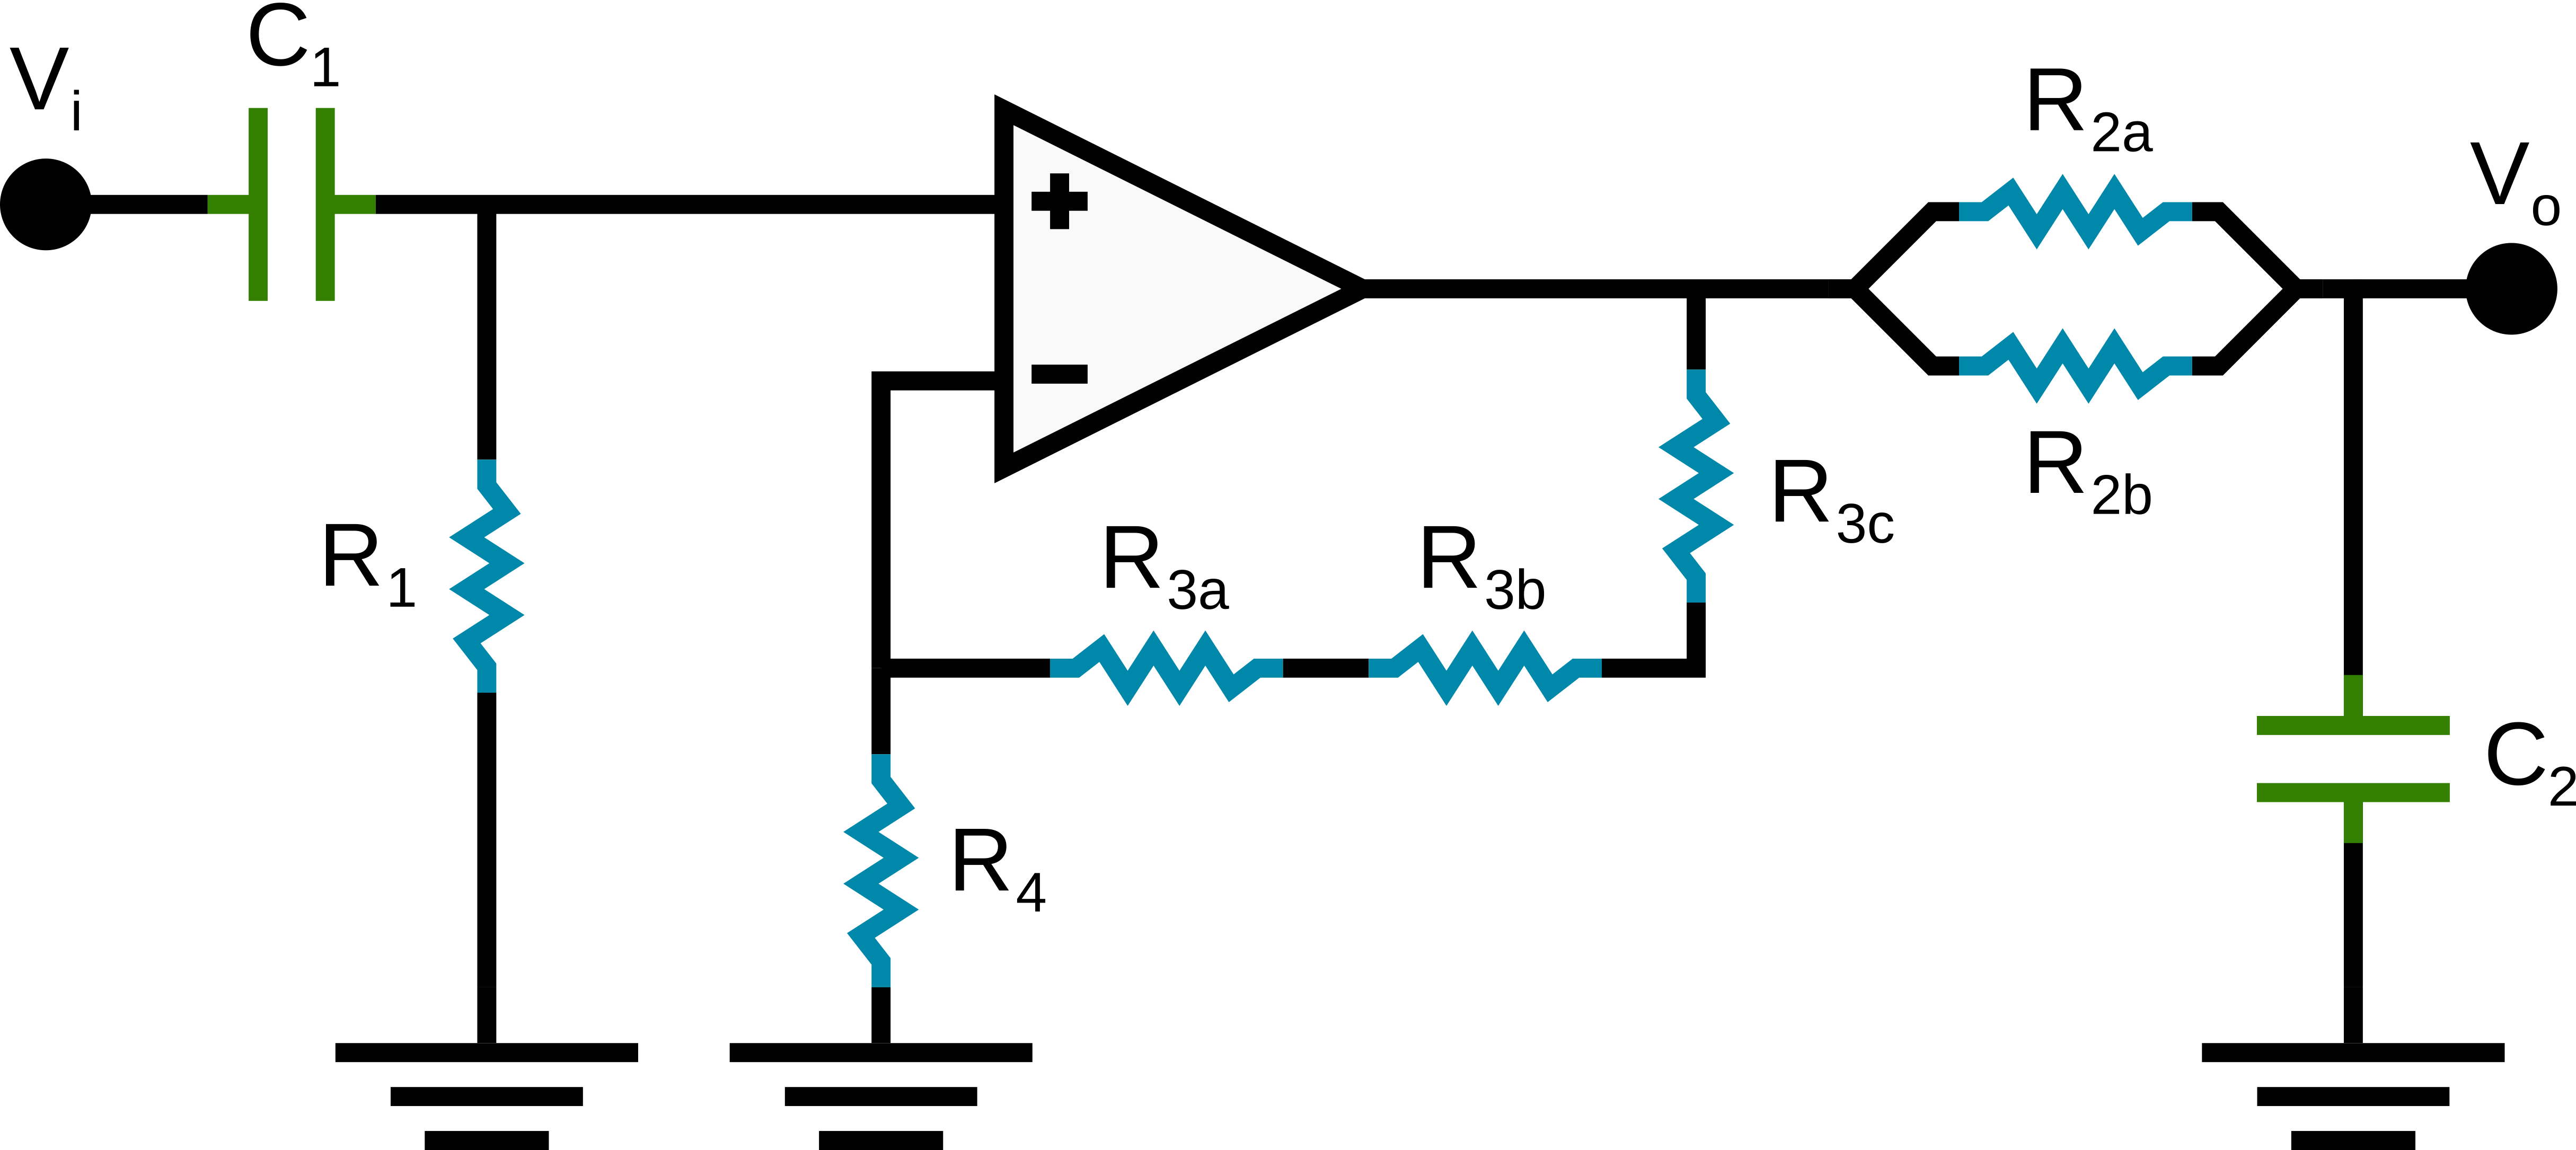
\includegraphics[width=\linewidth]{circuit.png}
  \vspace{1cm}
  \caption{Amplifier circuit}
  \label{fig:circuit}
  \hfill
\end{figure}


\FloatBarrier


\section{Theoretical Analysis}
\label{sec:analysis}

%As stated earlier, in this section, the theoretical analysis of the laboratory is made. These results were all obtained through GNU Octave.



\begin{Capacitor, C, as a open circuit} 
%The first point of the Theoretical analysis requested "asked" for a study of the node voltages for t<0, that is, for a constant voltage signal, at the voltage source, Vs. 


\end{align*}


[filler]
[filler]


$$
\begin{bmatrix} 
[filler]
[filler]
\end {bmatrix} 
\begin{bmatrix} 
[filler]
[filler]
\end {bmatrix} 
=
\begin{bmatrix} 
[filler]
[filler]
\end {bmatrix} 
$$


[filler]
[filler]

\begin{align*} 
[filler]
[filler]
\end{align*}

 

[filler]
[filler]



\begin{align*} 
[filler]
[filler]
\end{align*}

[filler]
[filler]

\begin{align*} 
[filler]
[filler]
\end{align*}

[filler]
[filler]


$$
\begin{bmatrix} 
[filler]
[filler]
\end {bmatrix} 
\begin{bmatrix}
[filler]
[filler]
\end{bmatrix}
=
\begin{bmatrix}
[filler]
[filler]
\end{bmatrix}
$$


[filler]
[filler]
[filler]
[filler]


%\FloatBarrier
%\begin{table}[h]
%  \centering
%  \begin{tabular}{|c|c|c|c|c|c|c|}
%    \hline    
%    
 V(1) & V(2) & V(3) & V(4) & V(5) & V(6) & V(7) \\ 
 5.24841 V   & 4.9997 V  & 4.47559 V  & 5.03486 V  & 5.80216 V  & -1.97226 V  & -2.96144 V\\

%    \hline
%  \end{tabular}
%  \caption{Nodal method}
%  \label{tab:nodal}
%\end{table}
%\FloatBarrier

%\FloatBarrier
%\begin{table}[h]
%  \centering
%  \begin{tabular}{|c|c|c|c|}
%   \hline    
%   \input{mesh}
%    \hline
%  \end{tabular}
%  \caption{Mesh method}
%  \label{tab:mesh}
%\end{table}
%\FloatBarrier


\section{Simulation Analysis}
\label{sec:simulation} 

From the AC sweep analysis, we obtained the following results for the frequency response:


%%%%%%%tabela das frequencias e gain
\begin{table}[!htb]
  \parbox{.45\linewidth}{
    \centering
    \begin{tabular}{|l|l|}
      \hline
      \input{resources/frequencies_tab.tex}
    \end{tabular}
    \caption{Lower and upper cutoff frequencies plus central frequency (in Hertz)}
  }
\hfill
  \parbox{0.45\linewidth}{
    \centering
    \begin{tabular}{|l|l|}
      \hline    
      \input{resources/maxgain_tab.tex}
    \end{tabular}
    \caption{Voltage gain in function of frequency (in dB and V/V)}
  }
\end{table}
%%%%%%%tabela das frequencias e gain

Where the gain is measured in V/V both at its peak overall, and at the central frequency of 1kHz.\\
The cuttoff frequencies are used to obtain the true central frequency so it can be compared to the target of 1kHz.\\ \\ \\

The following tables present the deviation of the gain and central frequency from their target of 100V/V (40dB) and 1kHz respectively, as well as the merit figure obtained for this design in function of its cost and performance.
%%%%%%%tabela dos desvios e do merito
\begin{table}[!htb]
\parbox{.45\linewidth}{
\centering
\begin{tabular}{|l|l|}
    \hline    
    \input{resources/deviations_tab.tex}
  \end{tabular}
  \caption{deviations}
}
\hfill
\parbox{.45\linewidth}{
\centering
\begin{tabular}{|l|l|}
    \hline    
    \input{resources/merit_tab.tex}
  \end{tabular}
  \caption{merit}
  \label{tab:Spice1}
}
\end{table}
%%%%%%%tabela dos desvios e do merito

The merit figure is quite poor. Unlike previous lab assignments, we were not able to fully optimize this circuit due to the several possible designs that can be made, which would require several simulations and theoretical models to be developed until the best amplifier design could be found.\\ \\ \\

The input and output impedances were also simulated for the central target frequency of 1kHz and are presented in the following tables. 


\begin{table}[!htb]
\parbox{.45\linewidth}{
  \centering
  \begin{tabular}{|l|l|}
    \hline    
    \input{resources/outputimped_tab.tex}
  \end{tabular}
  \caption{Output Impedace}
}
\hfill
\parbox{.45\linewidth}{
  \centering
  \begin{tabular}{|l|l|}
    \hline    
    \input{resources/inputimped_tab.tex}
  \end{tabular}
  \caption{Input Impedace}
}
\end{table}




\FloatBarrier  
\begin{figure} [!htb] 
  \includegraphics[trim={0 45px 0 230px},width=\linewidth]{resources/gain.pdf}
  \caption{Gain}
  \label{fig:theoplots}
  \hfill
\end{figure}

\begin{figure} [!htb] 
  \minipage{0.9\textwidth}
  \includegraphics[width=\linewidth]{resources/phase.pdf}
  \caption{Phase}
  \label{fig:theoplots}
  \endminipage
  \hfill
\end{figure}
\FloatBarrier


%Escrever como as incrementações nos valores influenciam por exemplo a utilização de um condensador e consequentemente a resistência do mesmo no gain voltage
 

\section{Comparisons}
\label{sec:comparsisons}

In this section, a comparision between the ngspice and octave results is made. Moreover, we delve into the reasons regarding the diffences and similarities observed\\
Starting with the frequency response, the gain and phase are presented bellow.\\
\FloatBarrier
Gain:


\begin{figure} [!htb] 
	\begin{subfigure}[b]{0.5\textwidth}
		\centering
  		\includegraphics[width=\textwidth]{resources/gain.pdf}
  		\caption{NGspice voltage gain}
	\end{subfigure}
  	\begin{subfigure}[b]{0.5\textwidth}
  		\centering
 		 \includegraphics[width=\textwidth]{resources/gain.png}
 		 \caption{Octave voltage gain}
  	\end{subfigure}
\end{figure}
\FloatBarrier
\FloatBarrier
Phase:


\begin{figure} [!htb] 
	\begin{subfigure}[b]{0.5\textwidth}
 		 \includegraphics[width=\textwidth]{resources/phase.pdf}
  		\caption{NGspice voltage phase}
 		\label{fig:theoplots}
	\end{subfigure}
  	\begin{subfigure}[b]{0.5\textwidth}
  		\includegraphics[width=\textwidth]{resources/phase_deg.png}
 		 \caption{Octave voltage phase}
 		 \label{fig:theoplots}
  	\end{subfigure}
\end{figure}
\FloatBarrier




In the following tables, the input and ouput inpedances  calculated at the central frequency from both analysis are presented.

%\FloatBarrier
%\begin{table}[h]
%  \centering
%  \begin{tabular}{|c|c|c|}
%    \hline    
%    \input{}
%    \hline
%  \end{tabular}
%  \caption{Input Impedance by Ngspice}
%  \label{tab:Spice1}
%\end{table}
%\FloatBarrier   

\FloatBarrier
\begin{table}[h]
  \centering
  \begin{tabular}{|c|c|c|}
    \hline    
    \input{resources/Z.tex}
    \hline
  \end{tabular}
  \caption{Input and Output Impedances by Octave}
  \label{tab:Spice1}
\end{table}
\FloatBarrier   

%The cost of the design is: \input{}\\




\section{Conclusion}
\label{sec:conclusion} 
During the course of this Lab, an amplifier with bandpass filter was designed, simulated and theoretically analysed. The theoretical model proved to be faithful to the simulation regarding the calculation of the central frequency, as well the gain estimation for a band of frequencies; there were deviations, but of small magnitude. It was, however, a subpar model for calculating the input and output impedances of the circuit, since there were noticeable deviations between the theoretical values and the simulated ones.\\
Due to the limitations imposed on the number and type of components that could be used, the center frequency wasn't exactly 1kHz. The central frequency goal also imposed a limitation, namely on the impedances. Since the resistors R2 and R1 as well as the capacitators had to be chosen with this goal in mind the output impedance couldn't be lowered.\\
The final design was able to produce a gain of 2.067604e+01 volts at a central frequency of 9.030675e+02 Hz.\\



% ----------------------------------------------------------------------
%  Bibliography
% ----------------------------------------------------------------------
%\addcontentsline{toc}{section}{\bibname}
%\bibliographystyle{abbrvunsrtnat} % <<<<< SELECT IF USING REFERENCES BY NUMBER (CITATION ORDER)
%\bibliography{../../../BIBfile.bib}
\begin{thebibliography}{9}

\bibitem{codecs}
K. Mayaram (1988) in 'DC and transient analyses'
\textit{CODECS: A Mixed-Level Circuit and Device Simulator, Memorandum No. UCB/ERL M88/71} Berkeley , p.23
\\\texttt{http://www.eecs.berkeley.edu/Pubs/TechRpts/1988/ERL-88-71.pdf}
\end{thebibliography}
% ----------------------------------------------------------------------
\end{document}
% ----------------------------------------------------------------------

